\documentclass{article}
\usepackage[utf8x]{inputenc}
\usepackage{ucs}
\usepackage{amsmath} 
\usepackage{amsfonts}
\usepackage{upgreek}
\usepackage[english,russian]{babel}
\usepackage{graphicx}
\usepackage{float}
\usepackage{textcomp}
\usepackage{hyperref}
\usepackage{geometry}
  \geometry{left=2cm}
  \geometry{right=1.5cm}
  \geometry{top=1cm}
  \geometry{bottom=2cm}
\usepackage{tikz}
\usepackage{ccaption}
\usepackage{multicol}

\usepackage{listings}
%\setlength{\columnsep}{1.5cm}
%\setlength{\columnseprule}{0.2pt}


\begin{document}
\pagenumbering{gobble}

\lstset{
  language=C,                % choose the language of the code
  basicstyle=\linespread{1.1}\ttfamily,
  columns=fixed,
  fontadjust=true,
  basewidth=0.5em,
  keywordstyle=\color{blue}\bfseries,
  commentstyle=\color{gray},
  stringstyle=\ttfamily\color{orange!50!black},
  showstringspaces=false,
  %numbers=false,                   % where to put the line-numbers
  numbersep=5pt,
  numberstyle=\tiny\color{black},
  numberfirstline=true,
  stepnumber=1,                   % the step between two line-numbers.        
  numbersep=10pt,                  % how far the line-numbers are from the code
  backgroundcolor=\color{white},  % choose the background color. You must add \usepackage{color}
  showstringspaces=false,         % underline spaces within strings
  captionpos=b,                   % sets the caption-position to bottom
  breaklines=true,                % sets automatic line breaking
  breakatwhitespace=true,         % sets if automatic breaks should only happen at whitespace
  xleftmargin=.2in,
  extendedchars=\true,
  keepspaces = true,
}
\lstset{literate=%
   *{0}{{{\color{red!20!violet}0}}}1
    {1}{{{\color{red!20!violet}1}}}1
    {2}{{{\color{red!20!violet}2}}}1
    {3}{{{\color{red!20!violet}3}}}1
    {4}{{{\color{red!20!violet}4}}}1
    {5}{{{\color{red!20!violet}5}}}1
    {6}{{{\color{red!20!violet}6}}}1
    {7}{{{\color{red!20!violet}7}}}1
    {8}{{{\color{red!20!violet}8}}}1
    {9}{{{\color{red!20!violet}9}}}1
}


\section*{Работа с терминалом:}
\subsection*{Основные команды:}
\texttt{
\begin{tabular}{ c | c }
 pwd                     & напечатать имя текущей директории \\ 
 ls                      &  напечатать все файлы и папки текущей директории \\ 
 ls -l                   &  то же, что и ls, но больше информации о файлах \\
 cd <имя папки>          & перейти в соответствующую папку \\
                         & например:  cd /home-local/student \\
 mkdir <имя новой папки> & создать новую папку \\
 cp <путь до файла> <путь до копии> & скопировать файл \\
 mv <путь до файла> <новый путь>    & переместить файл \\
 rm <путь до файла>                 & удалить файл \\
 rm -r <путь до папки>              & удалить папку \\
 nano <имя файла>                   & nano - это простейший текстовый редактор\\
                                    & открывает соответствующий файл, если его нет, то создаёт его\\
                                    & Ctrl-O - сохранить;  Ctrl-W - выйти\\
\end{tabular}
}
\subsection*{Сокращение директорий:}
\texttt{
\begin{tabular}{ c | c }
 /                       & корневая директория \\ 
 .                       & текущая директория \\ 
 ..                      & директория, которая содержит текущую \\ 
 \texttildelow                       & директория пользователя (/home-local/student) \\
\end{tabular}
}

\subsection*{Горячие клавиши:}
\texttt{
\begin{tabular}{ c | c }
 Tab           & автозаполнение \\ 
 2 раза Tab    & показать возможные варианты \\ 
 стрелка вверх & перейти к предыдущей команде \\ 
 Ctrl-C        & выход из программы, например той, которая зависла \\ 
 Ctrl-R        & поиск по всем предыдущим командам \\ 
\end{tabular}
}

\subsection*{Задание 1:}
\begin{enumerate}
\item Откройте терминал и перейдите в папку  \texttt{/home-local/student}
\item Создайте вашу папку, в которой вы будете работать в течении семестра.
\item Перейдите в эту папку и создайте там файл \texttt{test.txt}
\item Откройте этот файл с помощью \texttt{nano} и напишите в нём что-либо (на ваше усмотрение)
\item Скопируйте этот файл в эту же директорию, но под другим именем.
\item Создайте новую директорию и скопируйте туда файл \texttt{test.txt}
\item Переименуйте файл \texttt{test.txt}
\item Перейдите в новую созданную вами папку
\item Откройте файл из этой папку в \texttt{nano} и измените его.
\item Выйдите из этой папки (перейдите выше:  \texttt{cd ..})
\item Зайдите в вашу папку в файловом менеджере (``проводнике'') и проверьте всё.
\item Удалить созданные файлы в терминале с помощью \texttt{rm}
\end{enumerate}

\subsection*{Компиляция программы:}
Простейшая программа на языке C выглядит следующим образом:
\begin{lstlisting}
#include <stdio.h>
int main() 
{
    printf("Hello world!");
}
\end{lstlisting}

Эта программа печатает на экран строку "Hello world!".
\begin{itemize}
\item \texttt{\#include <stdio.h>}  - включаем библиотеку stdio (standard input/output), которая содержит функцию \texttt{printf}.
\item \texttt{int main() \{ ... \}} - основная функция программы, с неё начинается исполнение любой программы.
\item \texttt{printf("Hello world!");} - печатаем на экран.
\end{itemize}

Любая программа на языке C должна содержать особую функцию под названием main. По аналогии с обычными математическими функциями, функции в языке C могут принимать и возвращать значения. Принимаемые значения указываются в круглых скобках(в данном случае там ничего нет так как функция ничего не принимает) а тип возвращаемого значения указывается перед функцией (для функции main это всегда тип int, т.е. Integer - т.е. целое число). В фигурных скобках описываются операции, которые совершает функция. 
\subsection*{Компилятор \texttt{gcc}:}


\texttt{
\begin{tabular}{ c | c }
 gcc <имя файла исходного кода>  & скомпилировать программу и создать исполняемый файл \texttt{a.out} \\ 
                                 & файл исходного кода должен иметь расширение \texttt{.c} \\
 <путь до исполняемого файла>    & запустить исполняемый файл \\
 ./a.out                         & например, запустить файл a.out в текущей директории \\ 
                                 & . - текущая директория; a.out - имя файла \\ 
 gcc -o <исполняемый файл> <.c файл>  & скомпилировать программу и создать исполняемый файл \\
 gcc -std=c99 <.c файл>  & использовать стандарт языка C 99-го года (современный) \\
 gcc -lm <.c файл>  & подключить математическую библиотеку (если вы используете math.h) \\
\end{tabular}
}
\\
\begin{center}
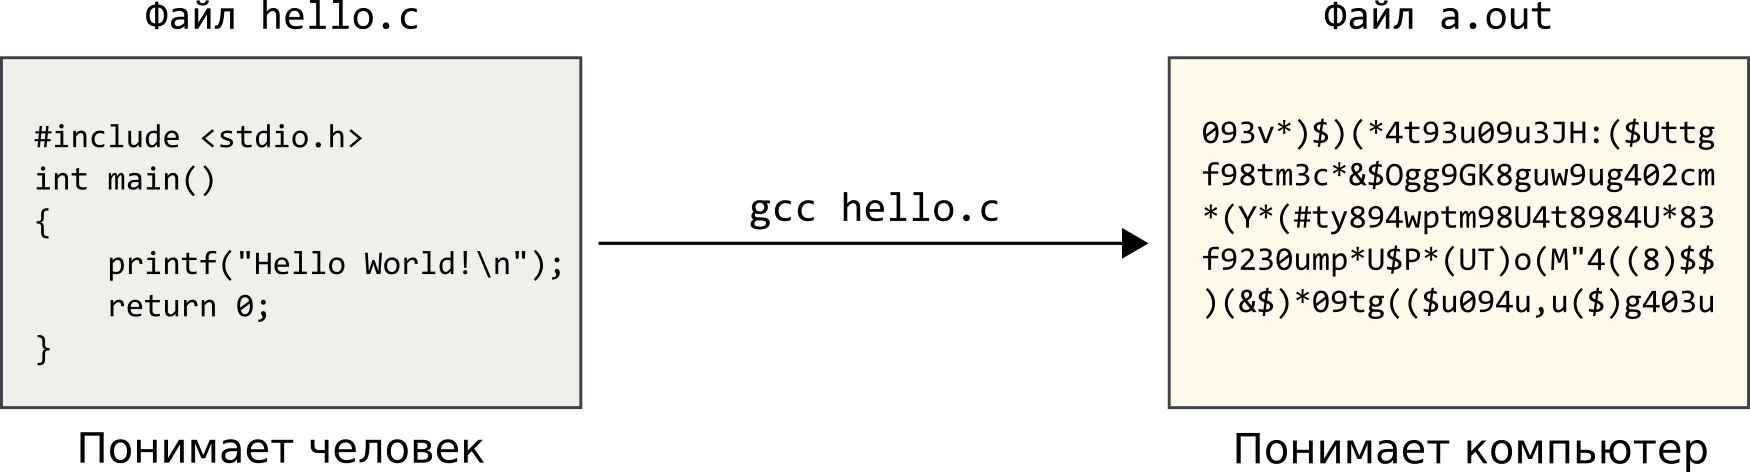
\includegraphics[scale=1]{../images/gcc_simple.png}
\end{center}
Таким образом, чтобы скомпилировать и запустить файл \texttt{hello.c} в исполняемый файл \texttt{hello} в нужном стандарте и с подключённой математической библиотекой нужно написать:
\begin{verbatim}
gcc -o hello -std=c99 -lm hello.c
./hello
\end{verbatim}
или так:
\begin{verbatim}
gcc -o hello -std=c99 -lm hello.c  &&  ./hello
\end{verbatim}
Помните, что постоянно набирать эту команду не надо, можно просто использовать стрелку вверх.
\begin{center}
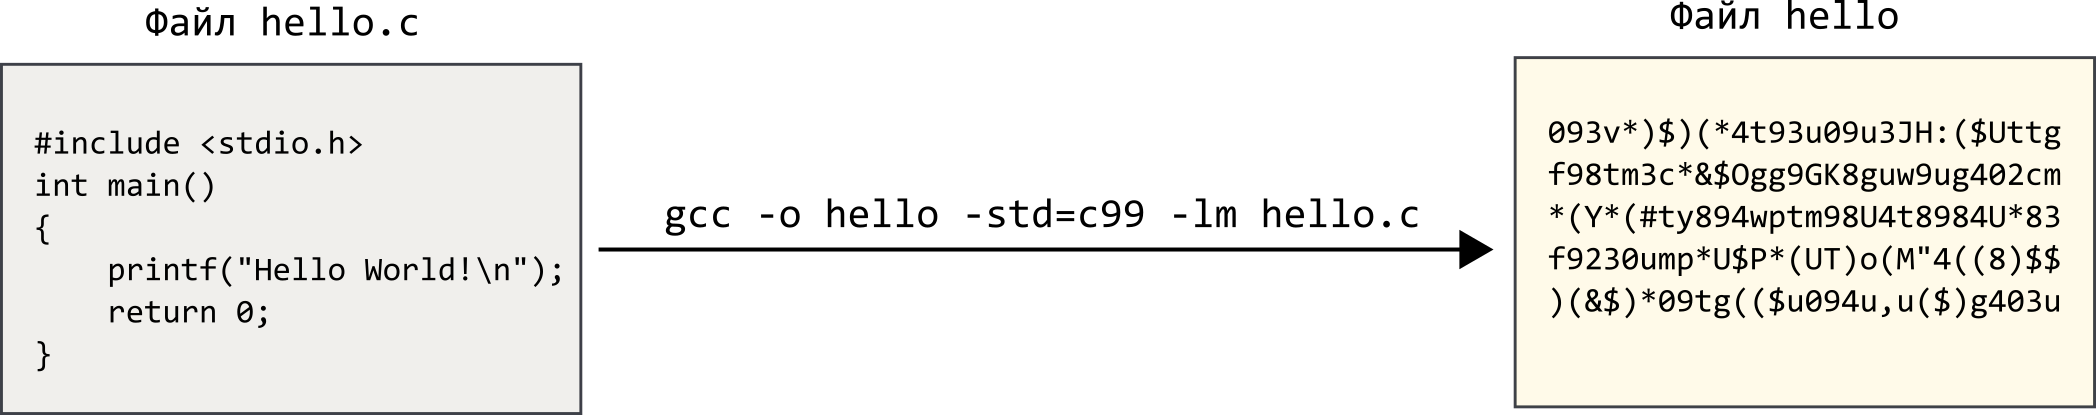
\includegraphics[scale=1]{../images/gcc_complex.png}
\end{center}

\subsubsection*{Задание 2:}
\begin{enumerate}
\item Скомпилируйте программу \texttt{hello.c} и запустите файл \texttt{a.out}.
\item Скомпилируйте программу \texttt{hello.c} с опцией \texttt{-o} и запустите файл \texttt{hello}.
\item В строке функции \texttt{printf()} можно использовать некоторые специальные символы \textbackslash n, \textbackslash t и \textbackslash b. Добавьте эти символы в строку функции printf и выясните, что они делают.
\end{enumerate}

\section*{Переменные \texttt{int} (целое число) и их печать - printf:}
В переменных \texttt{int} можно хранить целые числа от $-2^{31}$ до $2^{31} - 1$. ($2^{31}$ примерно равно двум миллиардам)
\begin{lstlisting}
#include <stdio.h>
int main() 
{
    int a;
    int b = 5;
    a = 3;
    int res = a * b + (b / a);
    printf("Result = %i\n", res);
}
\end{lstlisting}

\begin{itemize}
\item \texttt{int a} - Объявляем, что у нас есть переменная a, которая будет хранить целые числа (от англ. integer - целое число).
\item \texttt{int b = 5} - Объявляем, что у нас есть переменная b, которая будет хранить целые числа и присваиваем ей число 5.
\item \texttt{a = 3} - Присваиваем переменной a число 3.
\item \texttt{res = a * b + (b / a)} - Сохраняем в переменной res результат вычислений.
\item \texttt{printf(``Result = \%i \textbackslash n '', res)} Печатаем, за место спецификатора \texttt{\%i} (сокращение от \texttt{int}) подставится значение переменной.
\end{itemize}
\subsubsection*{Задание 2:}
\begin{enumerate}
\item Пусть \texttt{a = 451}. Напечатать \texttt{a} с помощью следующих спецификаторов:
\begin{multicols}{3}
	\begin{itemize}
	\item \texttt{\%i}
	\item \texttt{\%d}
	\item \texttt{\%7d}
	\item \texttt{\%07d}
	\item \texttt{\%x}
	\item \texttt{\%X}
	\item \texttt{\%o}
	\end{itemize}
\end{multicols}
\item Пусть \texttt{a = 436596}, а \texttt{b = 7361}. Найти и напечатать остаток деления \texttt{a} на \texttt{b}. Остаток вычисляется с помощью оператора \texttt{a \% b}.
\item Пусть \texttt{a = 2147483647} (максимальное возможное значение для \texttt{int}). Напечатайте значение \texttt{a + 1} и \texttt{2a}.

\end{enumerate}

\section*{Адрес и размер переменной:}
\begin{itemize}
\item 1 бит - минимальная единица измерения памяти. В 1 бите может хранится либо \texttt{0} либо \texttt{1}.
\item Вся память делится на ячейки, размером в 8 бит = 1 байт.
\item Все эти ячейки занумерованы, номер ячейки называется адресом.
\item Все переменные содержатся в памяти. Адрес переменной - это адрес первого байта переменной.
\item Чтобы найти адрес переменной, нужно перед ней поставить \texttt{\&}, например, \texttt{\&a}
\item Чтобы найти размер переменной в байтах: \texttt{sizeof(a)}
\item Например, переменная типа \texttt{int} имеет размер 4 байта = 32 бита. Значит в ней может хранится максимум $2^{32}$ значений.
\end{itemize}

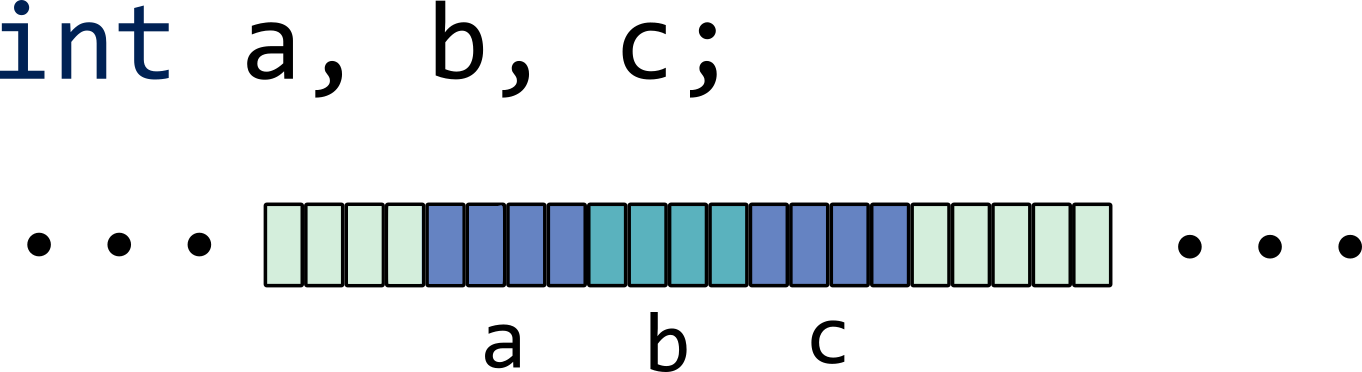
\includegraphics[scale=0.8]{../images/memory_ints.png}

\subsubsection*{Задание 3:}
\begin{enumerate}
\item Создать целочисленные переменные типов \texttt{int}, \texttt{short} и \texttt{char}. Напечатать их адрес и размер.
\end{enumerate}

\section*{Считывание переменных - scanf:}
Считывание переменных из терминала осуществляется с помощью функции \texttt{scanf} из библиотеки \texttt{stdio}. В отличии от \texttt{printf}, в \texttt{scanf} нужно передавать не саму переменную, а её адрес. Это естественно, так как \texttt{scanf} должен записать считываемое значение в соответствующие ячейки памяти.\\
Пример программы, которая считывает переменные a и b и печатает их на экран:
\begin{lstlisting}
#include <stdio.h>
int main() 
{
    int a, b;
    scanf("%i", &a); // <-- не забудьте тут амперсанд &
    scanf("%i", &b); // <-- не забудьте тут амперсанд &
    printf("Multiplication = %i\n", a * b);
}
\end{lstlisting}
\subsubsection*{Задание 4:}
\begin{enumerate}
\item Считать 2 целых числа и напечатать результат целочисленного деления первого на второе. Считать 2 числа с помощью \texttt{scanf} можно и одной строкой: \texttt{scanf(``\%i\%i'', \&a, \&b)}.
\item Считать 2 целых числа и напечатать остаток деления первого на второе.
\item На вход подаётся прошедшее время в формате \texttt{hh:mm}, например, \texttt{05:14}. Нужно напечатать, общее количество минут. Создайте 2 переменные \texttt{hours} и \texttt{minutes} и считать значения этих переменных с помощью \texttt{scanf}. 
\item Операторы \texttt{++}. Чему будут равны результаты выполнения следующего кода. Напечатайте \texttt{a}, \texttt{b} и \texttt{c}.
\begin{lstlisting}
#include <stdio.h>
int main() {
    int a = 753;
    int b = a++;
    int c = ++a;
}
\end{lstlisting}
\end{enumerate}


\newpage
\section*{Вещественные числа:}
Пример программы, которая считывает 2 вещественных числа и вычисляет среднее геометрическое:
\begin{lstlisting}
#include <stdio.h>
#include <math.h>
int main() 
{
    float a, b;
    scanf("%f", &a); // <-- не забудьте тут амперсанд & и %f
    scanf("%f", &b); // <-- не забудьте тут амперсанд & и %f
    printf("Geometric average = %f\n", sqrt(a * b));
}
\end{lstlisting}
В библиотеке \texttt{math.h} хранятся математические функции, такие как \texttt{sqrt} (корень), \texttt{sin}, \texttt{cos}, \texttt{exp}, \texttt{log} (натуральный логарифм), \texttt{fabs} (модуль вещ. числа) и другие. 
\subsubsection*{Задание 5:}
\begin{enumerate}
\item На вход программе подаются 2 положительных вещественных числа - катеты треугольника. Найти гипотенузу.
\item На вход программе подаются 2 положительных вещественных числа \texttt{a} и \texttt{b}. Вычислить значение выражения \texttt{sin(|a - b|) + log(a + b)}.
\end{enumerate}
\section*{Логические операторы:}
Пример программы, использующие логические операторы:
\begin{lstlisting}
#include <stdio.h>
int main() 
{
    int age;
    scanf("%i", &age);
    if (age >= 18 && age < 28)
    	printf("Yes\n")
    else
    	printf("No\n")
}
\end{lstlisting}

\begin{center}
\texttt{\begin{multicols}{2}
\begin{tabular}{ c c }
 == & равно \\ 
 != & не равно \\  
 > & больше \\  
 >= & больше и равно \\ 
 < & меньше \\
 <= & меньше и равно \\
\end{tabular}
\begin{tabular}{ c c }
 \&\& & логическое И \\ 
 || & логическое ИЛИ \\  
 !  & логическое НЕ \\  
\end{tabular}
\end{multicols}
}
\end{center}
\subsubsection*{Задание 6:}
\begin{enumerate}
\item Написать программу, которая принимает на вход число и печатает \texttt{Positive}, если число положительное, \texttt{Negative}, если число отрицательное и \texttt{Zero}, если число равно нулю.
\item Написать программу, которая принимает на вход число и печатает \texttt{Yes}, если число принадлежит множеству $(-\infty, -12] \cup (97, +\infty)$.
\item Написать программу, которая принимает на вход число и печатает \texttt{Even}, если число четное и \texttt{Odd}, если число нечетное. Подсказка: \texttt{\%}.
\end{enumerate}

\section*{Цикл \texttt{while}:}
Пример: программа, которая вычисляет сумму чисел от \texttt{1} до \texttt{n}. Тело цикла \texttt{while} повторяется до тех пор, пока выполнено условие \texttt{n != 0}.
\begin{lstlisting}
#include <stdio.h>
int main() 
{
    int n;
    scanf("%d", &n);
    int sum = 0;
    while (n != 0)
    {
        sum += n;
        n--;
    }
    printf("%d\n", sum);
}
\end{lstlisting}
\subsubsection*{Задание 7:}
\begin{enumerate}
\item Написать программу, которая будет вычислять произведение всех чисел от \texttt{1} до \texttt{n}.
\item Написать программу, которая печатает все числа от 1 до n и их квадраты в следующем виде:
\begin{verbatim}
1 1
2 4
3 9
4 16
...
\end{verbatim}
\item Написать программу, которая будет печатать все числа от \texttt{1} до \texttt{n}, которые делятся на 7. (Подсказка: в данной задаче можно не использовать \texttt{\%}).
\item Написать программу, которая будет считывать \texttt{n} и печатать \texttt{n} звёздочек \texttt{*}.
\item Написать программу, которая будет проходить все числа от \texttt{1} до \texttt{n}. Если число делится на \texttt{3}, то программа должна печатать \texttt{Fizz}. Если число делится на \texttt{5}, то программа должна печатать \texttt{Buzz}. Если число делится на \texttt{3} и на \texttt{5}, то программа должна печатать \texttt{FizzBuzz}. Иначе программа должна печатать просто само число.
\item Написать программу, которая будет вычислять квадратный корень вавилонским способом. Считываем вещественное число \texttt{a} и нам нужно найти корень из него. Ищем следующим способом:
\begin{align*} 
&x_0 = 1\\
&x_n = \frac{1}{2}\Big(x_{n-1} + \frac{a}{x_{n-1}}\Big)
\end{align*}
Цикл заканчиваем когда выполнится условие: $|x_n - x_{n-1}| < 10^{-4}$.
\item Переписать предыдущие программы, используя цикл \texttt{for}.
\end{enumerate}
\end{document}